\documentclass[12pt,a4paper]{article}
\usepackage[a4paper, margin=0.8in, headheight=14pt]{geometry}
\usepackage{fontspec}
\usepackage{unicode-math}
\setmainfont{TeX Gyre Pagella}
\setmonofont[Scale=0.88]{TeX Gyre Cursor}
\setmathfont{Latin Modern Math}
\usepackage{xcolor}
\usepackage{colortbl}
\usepackage{titlesec}
\usepackage{enumitem}
\usepackage{tabularx}
\usepackage{booktabs}
\usepackage{array}
\usepackage{amsmath}
\usepackage{tikz}
\usetikzlibrary{shapes.geometric, arrows.meta, positioning, calc, fit, decorations.pathreplacing}
\usepackage{tcolorbox}
\tcbuselibrary{skins, breakable}
\usepackage{hyperref}
\usepackage{fancyhdr}
\usepackage{graphicx}
\usepackage{microtype}
\hyphenpenalty=10000
\exhyphenpenalty=10000
\sloppy
\usepackage{caption}
\usepackage{setspace}
\usepackage{multirow}
\usepackage{tocloft}
\newcommand{\Q}[1]{\textbf{#1}\par\noindent\ignorespaces}
\definecolor{myred}{RGB}{196,30,58}
\definecolor{mydark}{RGB}{30,30,50}
\definecolor{mygreen}{RGB}{14,120,80}
\definecolor{myteal}{RGB}{0,130,140}
\definecolor{myamber}{RGB}{180,100,0}
\definecolor{mypurple}{RGB}{100,30,160}
\definecolor{mygray}{RGB}{246,247,249}
\definecolor{mgframe}{RGB}{180,185,200}
\definecolor{watermark}{RGB}{145,150,170}
\definecolor{hdrred}{RGB}{250,232,235}
\definecolor{hdrgreen}{RGB}{220,244,233}
\definecolor{hdrteal}{RGB}{220,242,244}
\definecolor{hdramber}{RGB}{253,242,215}
\definecolor{hdrpurple}{RGB}{238,228,255}
\definecolor{hdrgray}{RGB}{238,240,245}
\definecolor{rowalt}{RGB}{250,251,253}
\titleformat{\section}{\large\bfseries\color{myred}}{\thesection.}{0.5em}{}[\vspace{1pt}{\color{myred}\rule{\linewidth}{0.8pt}}]
\titleformat{\subsection}{\normalsize\bfseries\color{myteal}}{\thesubsection}{0.5em}{}
\titlespacing*{\section}{0pt}{18pt}{7pt}
\titlespacing*{\subsection}{0pt}{11pt}{4pt}
\setlength{\parindent}{0pt}
\setlength{\parskip}{4pt}
\renewcommand{\cfttoctitlefont}{\large\bfseries\color{myred}}
\renewcommand{\cftaftertoctitle}{\par\noindent{\color{myred}\rule{\linewidth}{0.8pt}}}
\setlength{\cftbeforetoctitleskip}{0pt}
\setlength{\cftaftertoctitleskip}{6pt}
\renewcommand{\cftsecfont}{\normalsize\bfseries\color{mydark}}
\renewcommand{\cftsecpagefont}{\normalsize\bfseries\color{mydark}}
\renewcommand{\cftsecleader}{\cftdotfill{\cftdotsep}}
\setlength{\cftbeforesecskip}{7pt}
\renewcommand{\cftsubsecfont}{\small\color{mydark}}
\renewcommand{\cftsubsecpagefont}{\small\color{mydark}}
\setlength{\cftbeforesubsecskip}{3pt}
\setlength{\cftsubsecindent}{1.4em}
\renewcommand{\arraystretch}{1.45}
\setlength{\tabcolsep}{6pt}
\arrayrulecolor{mydark}
\newcolumntype{B}[1]{>{\small\bfseries\raggedright\arraybackslash}m{#1}}
\newcolumntype{Y}{>{\small\raggedright\arraybackslash}X}
\renewcommand{\tabularxcolumn}[1]{m{#1}}
\pagestyle{fancy}
\fancyhf{}
\fancyhead[L]{\small\color{myred}\textbf{PE-EC801B}\;\color{mydark}--- Fiber Optic Communication}
\fancyhead[R]{\small\color{myteal}\textbf{Module 5 Notes}}
\fancyfoot[C]{\small\color{mydark}\thepage}
\fancyfoot[R]{\small\color{watermark}\textit{\copyright\ Biraj}}
\renewcommand{\headrulewidth}{0.5pt}
\renewcommand{\footrulewidth}{0.3pt}
\hypersetup{colorlinks=true, linkcolor=myteal, urlcolor=myteal,
  pdfauthor={Biraj Sarkar}, pdftitle={PE-EC801B --- Module 5 Notes}}
\tcbset{
  tikzbox/.style={colback=mygray, colframe=mgframe, boxrule=0.6pt, arc=4pt,
    left=8pt, right=8pt, top=6pt, bottom=6pt,
    colbacktitle=mgframe, coltitle=mydark, fonttitle=\small\bfseries},
  defbox/.style={colback=hdrgreen, colframe=mygreen, boxrule=0.8pt, arc=4pt,
    left=9pt, right=9pt, top=6pt, bottom=6pt,
    colbacktitle=mygreen, coltitle=white, fonttitle=\small\bfseries},
  formulabox/.style={colback=hdrteal, colframe=myteal, boxrule=0.8pt, arc=4pt,
    left=9pt, right=9pt, top=7pt, bottom=7pt,
    colbacktitle=myteal, coltitle=white, fonttitle=\small\bfseries},
  examplebox/.style={colback=hdramber, colframe=myamber, boxrule=0.8pt, arc=4pt,
    left=9pt, right=9pt, top=6pt, bottom=6pt,
    colbacktitle=myamber, coltitle=white, fonttitle=\small\bfseries},
  masonbox/.style={colback=hdrpurple, colframe=mypurple, boxrule=0.8pt, arc=4pt,
    left=9pt, right=9pt, top=6pt, bottom=6pt,
    colbacktitle=mypurple, coltitle=white, fonttitle=\small\bfseries},
  exambox/.style={colback=hdrpurple, colframe=mypurple, boxrule=1pt, arc=5pt,
    left=10pt, right=10pt, top=8pt, bottom=8pt,
    colbacktitle=mypurple, coltitle=white, fonttitle=\bfseries,
    breakable, title after break={\textbf{Frequently Asked / Viva Questions (contd.)}}}
}
\tcbset{breakable}
\tikzset{
  block/.style={rectangle, draw=myteal, fill=hdrteal,
    text width=2.4cm, align=center, minimum height=0.95cm,
    font=\small, rounded corners=3pt, line width=0.7pt},
  redblock/.style={rectangle, draw=myred, fill=hdrred,
    text width=2.4cm, align=center, minimum height=0.95cm,
    font=\small, rounded corners=3pt, line width=0.7pt},
  netnode/.style={rectangle, draw=myteal, fill=hdrteal,
    text width=1.5cm, align=center, minimum height=0.8cm,
    font=\small, rounded corners=3pt, line width=0.7pt},
  sumjunc/.style={circle, draw=myamber, fill=hdramber,
    minimum size=0.62cm, font=\small, line width=0.8pt},
  snode/.style={circle, draw=mypurple, fill=hdrpurple,
    minimum size=0.55cm, font=\footnotesize, line width=0.7pt},
  arrow/.style={-Stealth, thick, color=mydark},
  redarrow/.style={-Stealth, thick, color=myred},
  line/.style={thick, color=mydark}
}

\begin{document}

\begin{center}
  {\LARGE\bfseries\color{myred} PE-EC801B --- Fiber Optic Communication}\\[5pt]
  {\normalsize\color{mydark} Semester VIII \quad$\bullet$\quad 3L:0T:0P \quad$\bullet$\quad 3 Credits}\\[3pt]
  {\normalsize\color{myteal}\textbf{Module 5 Exam Notes}}\\[3pt]
  {\small\color{mydark} CGEC \;$|$\; B.Tech ECE (2023--27) \;$|$\; \textit{Biraj Sarkar}}
\end{center}
\vspace{2pt}
\noindent{\color{myred}\rule{\linewidth}{1.5pt}}
\vspace{2pt}

\hypersetup{linkcolor=mydark}
\tableofcontents
\hypersetup{linkcolor=myteal}
\newpage

% ===============================================================================
\section{WDM Fundamentals}
% ===============================================================================

\begin{tcolorbox}[defbox, title={\textbf{Wavelength Division Multiplexing (WDM)}}]
\textbf{WDM} is a technology that multiplexes multiple optical carrier signals on a single fiber using different wavelengths (colors) of laser light. Each wavelength carries a separate data channel, dramatically multiplying the fiber capacity without laying additional fiber.
\end{tcolorbox}

\subsection{WDM Principle and ITU-T Channel Grid}
Multiple lasers operating at distinct wavelengths are combined (multiplexed) by a MUX onto a single fiber. At the far end, a DEMUX separates them back to individual receivers. Each wavelength channel is independent and carries its own data stream.

The \textbf{ITU-T G.694.1} standard defines the DWDM channel grid centered on 193.1\,THz (1552.52\,nm) with channel spacings of 12.5, 25, 50, or 100\,GHz.

\subsection{CWDM vs DWDM}
\par\noindent
{\renewcommand{\arraystretch}{1.55}
\begin{tabularx}{\linewidth}{|B{3.5cm}|Y|Y|}
\hline
\textbf{Parameter} & \textbf{CWDM} & \textbf{DWDM} \\
\hline
Full name & Coarse WDM & Dense WDM \\
\hline
Channel spacing & 20\,nm (ITU-T G.694.2) & 0.4--0.8\,nm (50--100\,GHz) \\
\hline
Channel count & 4--18 & 40--160+ \\
\hline
Wavelength range & 1271--1611\,nm & 1530--1565\,nm (C-band) \\
\hline
Laser requirement & Uncooled (no TEC) & Temperature-controlled (TEC) \\
\hline
Cost & Low & High \\
\hline
Amplification & No (too wide for EDFA) & EDFA compatible \\
\hline
Application & Metro, short-haul & Long-haul, backbone \\
\hline
\end{tabularx}}

% ===============================================================================
\section{WDM Components}
% ===============================================================================

\begin{tcolorbox}[defbox, title={\textbf{WDM MUX/DEMUX Devices}}]
WDM MUX combines multiple wavelengths onto one fiber; DEMUX separates them. Key technologies: Arrayed Waveguide Grating (AWG), Thin-Film Filter (TFF), and Fiber Bragg Grating (FBG).
\end{tcolorbox}

\subsection{Arrayed Waveguide Grating (AWG)}
An AWG is a planar integrated device with a star coupler at input, an array of waveguides of incrementally increasing lengths, and a second star coupler (phased array region). The path-length difference between adjacent waveguides is exactly one wavelength, causing different wavelengths to focus to different output ports due to constructive interference. AWGs are used for both MUX and DEMUX.

\textbf{Advantages:} Mass-producible on a single chip; very flat passband; bidirectional; scalable to 40+ channels. \textbf{Disadvantage:} Temperature-sensitive (requires TEC for DWDM).

\subsection{Thin-Film Filter (TFF)}
Uses multiple thin-film interference layers (Fabry-Perot cavity) to reflect one wavelength while transmitting all others. Stacked in series, each filter drops one channel. \textbf{Advantage:} Low insertion loss for the reflected channel, temperature stable. \textbf{Disadvantage:} Insertion loss accumulates for large channel counts.

\subsection{Fiber Bragg Grating (FBG)}
A periodic refractive index modulation written into the fiber core. Reflects only the Bragg wavelength $\lambda_B = 2n_{eff}\Lambda$ ($\Lambda$ = grating period) and transmits all others. Used with circulators for wavelength drop/add.

\begin{tcolorbox}[formulabox, title={\textbf{FBG Bragg Condition}}]
\[
\lambda_B = 2 n_{eff} \Lambda
\]
where $n_{eff}$ is the effective refractive index of the guided mode and $\Lambda$ is the grating period. Tunable by temperature or strain.
\end{tcolorbox}

\subsection{Optical Add-Drop Multiplexer (OADM)}
An OADM allows one or more wavelength channels to be dropped from and added to a WDM signal at an intermediate node without converting to electrical signals. A \textbf{ROADM} (Reconfigurable OADM) allows software-controlled selection of any channel.

\begin{tcolorbox}[tikzbox, title={WDM System Block Diagram --- 4-Channel DWDM}]
\centering
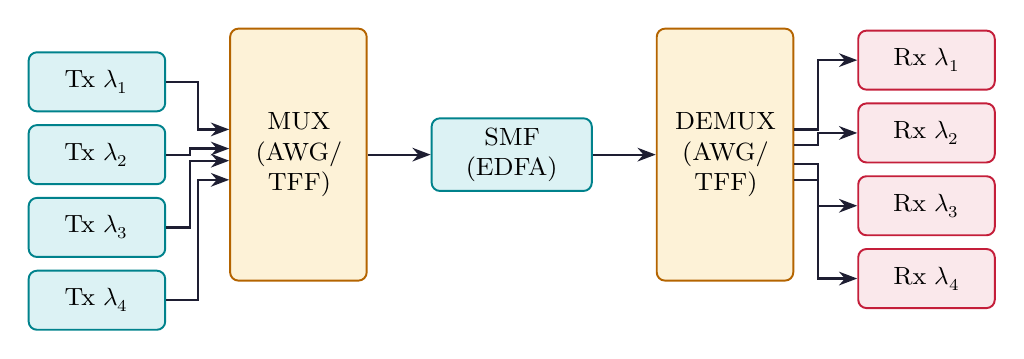
\begin{tikzpicture}[node distance=0.25cm and 0.45cm,
  sblock/.style={rectangle, draw=myteal, fill=hdrteal, text width=1.5cm,
    align=center, minimum height=0.75cm, font=\small, rounded corners=3pt, line width=0.7pt},
  rblock/.style={rectangle, draw=myred, fill=hdrred, text width=1.5cm,
    align=center, minimum height=0.75cm, font=\small, rounded corners=3pt, line width=0.7pt},
  mblock/.style={rectangle, draw=myamber, fill=hdramber, text width=1.5cm,
    align=center, minimum height=3.2cm, font=\small, rounded corners=3pt, line width=0.7pt}]
  % Transmitters
  \node[sblock] (tx1) {Tx $\lambda_1$};
  \node[sblock, below=0.15cm of tx1] (tx2) {Tx $\lambda_2$};
  \node[sblock, below=0.15cm of tx2] (tx3) {Tx $\lambda_3$};
  \node[sblock, below=0.15cm of tx3] (tx4) {Tx $\lambda_4$};
  % MUX
  \node[mblock, right=0.8cm of tx2] (mux) {MUX\\(AWG/\\TFF)};
  % Fiber
  \node[sblock, right=0.8cm of mux, minimum height=0.75cm, text width=1.8cm] (fiber) {SMF\\(EDFA)};
  % DEMUX
  \node[mblock, right=0.8cm of fiber] (demux) {DEMUX\\(AWG/\\TFF)};
  % Receivers
  \node[rblock, right=0.8cm of demux, yshift=1.2cm] (rx1) {Rx $\lambda_1$};
  \node[rblock, below=0.15cm of rx1] (rx2) {Rx $\lambda_2$};
  \node[rblock, below=0.15cm of rx2] (rx3) {Rx $\lambda_3$};
  \node[rblock, below=0.15cm of rx3] (rx4) {Rx $\lambda_4$};
  % Connections
  \draw[arrow] (tx1.east) -- ++(0.4,0) |- (mux.160);
  \draw[arrow] (tx2.east) -- ++(0.3,0) |- (mux.175);
  \draw[arrow] (tx3.east) -- ++(0.3,0) |- (mux.185);
  \draw[arrow] (tx4.east) -- ++(0.4,0) |- (mux.200);
  \draw[arrow] (mux.east) -- (fiber.west);
  \draw[arrow] (fiber.east) -- (demux.west);
  \draw[arrow] (demux.20) -- ++(0.3,0) |- (rx1.west);
  \draw[arrow] (demux.8) -- ++(0.3,0) |- (rx2.west);
  \draw[arrow] (demux.-8) -- ++(0.3,0) |- (rx3.west);
  \draw[arrow] (demux.-20) -- ++(0.3,0) |- (rx4.west);
\end{tikzpicture}
\end{tcolorbox}

% ===============================================================================
\section{WDM Network Principles --- OXC and Protection}
% ===============================================================================

\begin{tcolorbox}[defbox, title={\textbf{Optical Cross-Connect (OXC)}}]
An \textbf{OXC} is a network node that switches wavelength channels from any input fiber to any output fiber, entirely in the optical domain. It is the building block of all-optical mesh networks and enables wavelength routing.
\end{tcolorbox}

\textbf{Mesh topology and protection:}
\begin{itemize}[leftmargin=*, itemsep=3pt]
  \item \textbf{Mesh topology:} Each node connects to multiple other nodes via multiple fibers. Provides multiple routing paths for each wavelength channel.
  \item \textbf{Protection switching:} Dedicated 1+1 protection pre-assigns a backup path. On failure, traffic is immediately switched to backup ($<$50\,ms).
  \item \textbf{Restoration:} Dynamic rerouting of traffic around a failure using spare capacity. Takes longer ($>$100\,ms) but uses network resources more efficiently.
\end{itemize}

% ===============================================================================
\section{Nonlinear Effects in Optical Fiber}
% ===============================================================================

\begin{tcolorbox}[defbox, title={\textbf{Nonlinear Effects in Fiber}}]
At high optical power, the refractive index of silica becomes intensity-dependent: $n = n_0 + n_2 I$, where $n_2 \approx 2.6\times10^{-20}$\,m$^2$/W is the nonlinear refractive index coefficient. This gives rise to three key nonlinear phenomena: SPM, XPM, and FWM.
\end{tcolorbox}

\subsection{Self-Phase Modulation (SPM)}
A pulse modulates its own phase due to the intensity-dependent refractive index. The nonlinear phase shift accumulated is:
\[
\phi_{NL} = \gamma P_0 L_{eff}, \qquad \gamma = \frac{n_2 \omega}{c A_{eff}} = \frac{2\pi n_2}{\lambda A_{eff}}
\]
where $\gamma$ is the fiber nonlinearity coefficient, $P_0$ is peak power, $L_{eff}$ is the effective length.

\textbf{B-integral} (total accumulated nonlinear phase):
\[
B = \gamma P_0 L_{eff}
\]
SPM causes \textbf{spectral broadening} of the pulse. The leading edge of the pulse is red-shifted; the trailing edge is blue-shifted. In the anomalous dispersion regime, SPM and dispersion can balance to form solitons.

\subsection{Cross-Phase Modulation (XPM)}
In a WDM system, the intensity of one channel modulates the phase of an adjacent channel. The nonlinear phase induced in channel 2 by channel 1 is $2\gamma P_1 L_{eff}$ (factor of 2 due to polarization mixing). XPM causes amplitude-to-phase conversion, broadens spectra, and creates timing jitter in WDM channels.

\subsection{Four-Wave Mixing (FWM)}
When three channels at frequencies $\omega_1$, $\omega_2$, $\omega_3$ co-propagate, a new frequency $\omega_4 = \omega_1 + \omega_2 - \omega_3$ is generated (and other combinations). This creates crosstalk between WDM channels.

\begin{tcolorbox}[formulabox, title={\textbf{FWM Phase Matching Condition}}]
FWM is most efficient when the \textbf{phase mismatch} $\Delta\beta$ is small:
\[
\Delta\beta = \beta(\omega_1) + \beta(\omega_2) - \beta(\omega_3) - \beta(\omega_4) \approx 0
\]
In terms of the dispersion parameter $D$:
\[
\Delta\beta \approx \frac{2\pi c D}{\lambda^2} \Delta\lambda^2 \cdot \lambda^2
\]
FWM is strongest near the zero-dispersion wavelength (small $D$) and for equal channel spacing. Mitigation: use non-zero dispersion-shifted fiber (NZ-DSF) with $D \neq 0$ in the signal band.
\end{tcolorbox}

% ===============================================================================
\section{Group Velocity Dispersion (GVD) and Dispersion Parameter}
% ===============================================================================

\begin{tcolorbox}[defbox, title={\textbf{GVD and Dispersion Parameter $D$}}]
\textbf{Group velocity dispersion (GVD)} refers to the variation of group velocity with frequency, parameterized by $\beta_2 = d^2\beta/d\omega^2$ (ps$^2$/km). The \textbf{dispersion parameter} $D$ relates directly to $\beta_2$:
$D = -\frac{2\pi c}{\lambda^2}\beta_2$ \quad (ps/nm$\cdot$km).
\end{tcolorbox}

\begin{itemize}[leftmargin=*, itemsep=3pt]
  \item \textbf{Normal dispersion:} $\beta_2 > 0$ ($D < 0$); shorter wavelengths travel faster; pulse broadens normally.
  \item \textbf{Anomalous dispersion:} $\beta_2 < 0$ ($D > 0$); longer wavelengths travel faster; enables soliton formation.
  \item \textbf{Zero-dispersion wavelength $\lambda_0$:} For standard SMF, $\lambda_0 \approx 1310$\,nm. In DSF, shifted to 1550\,nm.
\end{itemize}

\begin{tcolorbox}[formulabox, title={\textbf{Dispersion Length}}]
\[
L_D = \frac{T_0^2}{|\beta_2|}
\]
where $T_0$ is the initial pulse half-width (1/e point). $L_D$ is the length at which the pulse broadens by $\sqrt{2}$. For $L \ll L_D$, dispersion is negligible.
\end{tcolorbox}

% ===============================================================================
\section{Soliton-Based Communication}
% ===============================================================================

\begin{tcolorbox}[defbox, title={\textbf{Optical Soliton}}]
An \textbf{optical soliton} is a pulse that propagates through a dispersive fiber without changing its shape, because the effects of anomalous GVD (pulse spreading) are exactly balanced by SPM (pulse compression). Solitons are solutions to the Nonlinear Schr\"{o}dinger Equation (NLSE).
\end{tcolorbox}

\subsection{Nonlinear Schr\"{o}dinger Equation (NLSE)}
The propagation of an optical pulse in a fiber is governed by:
\[
j\frac{\partial A}{\partial z} - \frac{\beta_2}{2}\frac{\partial^2 A}{\partial T^2} + \gamma |A|^2 A = 0
\]
where $A(z,T)$ is the slowly-varying pulse envelope, $\beta_2 < 0$ for anomalous dispersion, and $\gamma$ is the nonlinear coefficient.

\subsection{Fundamental Soliton (N = 1)}
The fundamental soliton has the \textbf{sech} profile:
\[
A(0,T) = \sqrt{P_0}\,\text{sech}(T/T_0)
\]
The soliton condition relates dispersion and nonlinear lengths:
\begin{tcolorbox}[formulabox, title={\textbf{Soliton Condition and Width-Power Relation}}]
\[
L_D = L_{NL}, \quad \text{i.e.,} \quad \frac{T_0^2}{|\beta_2|} = \frac{1}{\gamma P_0}
\]
\[
\Rightarrow \quad P_0 = \frac{|\beta_2|}{\gamma T_0^2}
\]
The peak power required for a soliton increases as the pulse width $T_0$ decreases. For $T_0 = 10$\,ps, $|\beta_2| = 20$\,ps$^2$/km, $\gamma = 2$\,W$^{-1}$km$^{-1}$: $P_0 = 20/(2\times100) = 0.1$\,W.\\
Higher-order solitons ($N = 2, 3, \ldots$) periodically breathe (compress and expand) with soliton period $z_s = \pi L_D / 2$.
\end{tcolorbox}

\subsection{Advantages and Limitations of Soliton Communication}
\textbf{Advantages:}
\begin{itemize}[leftmargin=*, itemsep=2pt]
  \item Dispersion-free propagation: pulse shape preserved over trans-oceanic distances.
  \item Allows very high bit rates (sub-picosecond pulses).
  \item With periodic amplification, solitons can be maintained over global distances.
\end{itemize}

\textbf{Limitations:}
\begin{itemize}[leftmargin=*, itemsep=2pt]
  \item Requires anomalous dispersion ($D > 0$) throughout the link; problematic with DCF.
  \item Gordon-Haus jitter: ASE noise from amplifiers causes random timing jitter, limiting transmission distance.
  \item Soliton--soliton interaction: adjacent pulses at the same wavelength must be spaced $>5T_0$ apart.
  \item Requires precise control of launch power and pulse shape.
  \item Dispersion management (DM-solitons) is needed for WDM compatibility.
\end{itemize}

\begin{tcolorbox}[tikzbox, title={Soliton Propagation vs Normal Pulse Propagation}]
\centering
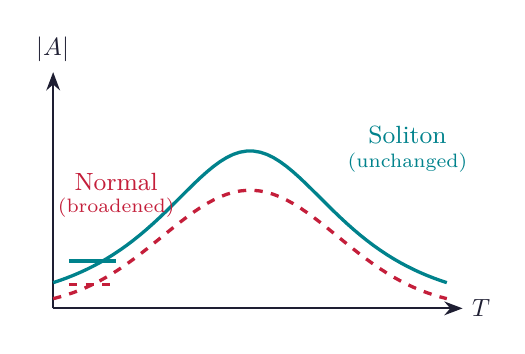
\begin{tikzpicture}[scale=1.0]
  \draw[-Stealth, thick, color=mydark] (0,0) -- (5.2,0) node[right,font=\small] {$T$};
  \draw[-Stealth, thick, color=mydark] (0,0) -- (0,3.0) node[above,font=\small] {$|A|$};
  % Soliton (sech profile, doesn't change)
  \draw[very thick, color=myteal, domain=-2.5:2.5, samples=60, variable=\t]
    plot ({2.5+\t}, {2.0/cosh(\t)});
  \node[font=\small\color{myteal}] at (4.5, 2.2) {Soliton};
  \node[font=\scriptsize\color{myteal}] at (4.5, 1.85) {(unchanged)};
  % Normal pulse (broadened Gaussian)
  \draw[very thick, color=myred, dashed, domain=-2.5:2.5, samples=60, variable=\t]
    plot ({2.5+\t}, {1.5*exp(-\t*\t/2.5)});
  \node[font=\small\color{myred}] at (0.8, 1.6) {Normal};
  \node[font=\scriptsize\color{myred}] at (0.8, 1.28) {(broadened)};
  % Legend
  \draw[very thick, color=myteal] (0.2,0.6) -- (0.8,0.6);
  \draw[very thick, color=myred, dashed] (0.2,0.3) -- (0.8,0.3);
\end{tikzpicture}
\end{tcolorbox}

% ===============================================================================
% QUICK REVISION PAGE
% ===============================================================================
\newpage
\begin{center}
  {\large\bfseries\color{myred} Quick Revision --- Module 5}\\[3pt]
  {\small\color{mydark} WDM Systems and Nonlinear Effects $|$ PE-EC801B}
\end{center}
\noindent{\color{myred}\rule{\linewidth}{1.2pt}}
\vspace{4pt}

\begin{tcolorbox}[formulabox, title={\textbf{Key Formulas at a Glance}}]
\renewcommand{\arraystretch}{1.35}
\begin{tabularx}{\linewidth}{B{5.0cm} X}
FBG Bragg condition & $\lambda_B = 2n_{eff}\Lambda$ \\[4pt]
SPM nonlinear phase & $\phi_{NL} = \gamma P_0 L_{eff}$ (B-integral) \\[4pt]
Fiber nonlinearity coeff. & $\gamma = 2\pi n_2 / (\lambda A_{eff})$ (W$^{-1}$km$^{-1}$) \\[4pt]
Dispersion parameter & $D = -(2\pi c/\lambda^2)\beta_2$ \quad (ps/nm$\cdot$km) \\[4pt]
Dispersion length & $L_D = T_0^2/|\beta_2|$ \\[4pt]
Nonlinear length & $L_{NL} = 1/(\gamma P_0)$ \\[4pt]
Soliton condition & $L_D = L_{NL}$ \\[4pt]
Soliton peak power & $P_0 = |\beta_2|/(\gamma T_0^2)$ \\[4pt]
Soliton shape & $A(0,T) = \sqrt{P_0}\,\text{sech}(T/T_0)$ \\[4pt]
DWDM channel spacing & 50--100\,GHz (ITU-T G.694.1) \\[4pt]
\end{tabularx}
\end{tcolorbox}

\begin{tcolorbox}[defbox, title={\textbf{One-Line Definitions}}]
\begin{itemize}[leftmargin=*, itemsep=2pt, topsep=0pt]
  \item \textbf{WDM:} Multiple wavelength channels on a single fiber; multiplies capacity without new fiber.
  \item \textbf{DWDM:} Dense WDM with 50/100\,GHz channel spacing; supports 40--160+ channels in C-band.
  \item \textbf{AWG:} Arrayed Waveguide Grating; planar integrated MUX/DEMUX using path-length differences.
  \item \textbf{FBG:} Fiber Bragg Grating; periodic index modulation reflecting only the Bragg wavelength.
  \item \textbf{OADM:} Optical Add-Drop Multiplexer; drops and adds wavelength channels at intermediate nodes.
  \item \textbf{OXC:} Optical Cross-Connect; switches wavelengths between fibers in an all-optical network node.
  \item \textbf{SPM:} Self-Phase Modulation; pulse modulates its own phase, causing spectral broadening.
  \item \textbf{XPM:} Cross-Phase Modulation; one WDM channel modulates the phase of another.
  \item \textbf{FWM:} Four-Wave Mixing; three channels generate a fourth frequency; crosstalk near $\lambda_0$.
  \item \textbf{Soliton:} Pulse that propagates undistorted due to exact SPM--GVD balance (anomalous dispersion).
  \item \textbf{$\beta_2$:} GVD parameter; $\beta_2 < 0$ = anomalous; $\beta_2 > 0$ = normal dispersion.
\end{itemize}
\end{tcolorbox}

\begin{tcolorbox}[exambox, title={\textbf{Frequently Asked / Viva Questions}}]
\begin{enumerate}[topsep=0pt, label=\textbf{Q\arabic*.}, itemsep=5pt]
  \item \Q{What is WDM and what are its advantages?}
    WDM multiplexes multiple wavelength channels on one fiber. Advantages: multiplies capacity $N$-fold without laying new fiber; each channel is protocol- and bit-rate-independent; can combine CWDM and DWDM in hybrid networks.
  \item \Q{Differentiate between CWDM and DWDM.}
    CWDM: 20\,nm channel spacing, 4--18 channels, 1271--1611\,nm, uncooled lasers, low cost, no EDFA. DWDM: 50--100\,GHz spacing, 40--160+ channels, 1530--1565\,nm, TEC-cooled lasers, EDFA-compatible, high capacity, high cost.
  \item \Q{What is an AWG and how does it work?}
    An Arrayed Waveguide Grating is a planar integrated optics device. Light enters a free propagation region (star coupler), splits into an array of waveguides with linearly increasing lengths, recombines in a second star coupler. The path-length differences cause different wavelengths to constructively interfere at different output ports.
  \item \Q{What is an FBG? State the Bragg condition.}
    A Fiber Bragg Grating is a periodic modulation of the refractive index written into the fiber core using UV light. It reflects only $\lambda_B = 2n_{eff}\Lambda$ and transmits all others. Used for channel dropping in OADMs, dispersion compensation, and sensing.
  \item \Q{What is Self-Phase Modulation? What does it cause?}
    SPM arises because $n = n_0 + n_2 I$. A pulse modulates its own phase: $\phi_{NL}(t) = \gamma P(t) L_{eff}$. The leading edge is red-shifted and trailing edge is blue-shifted, causing spectral broadening. In anomalous dispersion, SPM enables soliton formation.
  \item \Q{What is Four-Wave Mixing and when is it worst?}
    FWM generates new frequencies $\omega_4 = \omega_1 + \omega_2 - \omega_3$ from three co-propagating channels. It is worst when the phase mismatch $\Delta\beta \approx 0$, i.e., near the zero-dispersion wavelength $\lambda_0$. Equal channel spacing also maximizes FWM efficiency. NZ-DSF ($D \neq 0$) mitigates it.
  \item \Q{Define the dispersion parameter $D$ and state its units.}
    $D = -(2\pi c/\lambda^2)\beta_2$ in units of ps/nm$\cdot$km. It gives the pulse broadening per nm of source linewidth per km of fiber. Standard SMF: $D \approx +17$\,ps/nm$\cdot$km at 1550\,nm.
  \item \Q{What is anomalous dispersion and why is it needed for solitons?}
    Anomalous dispersion ($\beta_2 < 0$, $D > 0$): longer wavelengths travel faster. The chirp induced by anomalous GVD (red leading) is opposite to SPM chirp (red leading). At the right power, these two effects exactly cancel, producing a shape-invariant soliton.
  \item \Q{State the soliton condition and derive the soliton power.}
    Soliton condition: $L_D = L_{NL}$, i.e., $T_0^2/|\beta_2| = 1/(\gamma P_0)$. Solving: $P_0 = |\beta_2|/(\gamma T_0^2)$. For $T_0 = 10$\,ps, $|\beta_2| = 20$\,ps$^2$/km, $\gamma = 2$\,W$^{-1}$km$^{-1}$: $P_0 = 0.1$\,W.
  \item \Q{What are the limitations of soliton communication?}
    Gordon-Haus timing jitter (from ASE noise), soliton--soliton interaction requiring large pulse spacing ($>5T_0$), requirement for precisely anomalous dispersion throughout, and incompatibility with standard DWDM channels without dispersion-managed fiber.
  \item \Q{What is XPM and how does it differ from SPM?}
    XPM: the intensity of channel $i$ modifies the phase of channel $j$ with a coefficient of $2\gamma$ (vs $\gamma$ for SPM). XPM causes amplitude-dependent phase noise and timing jitter in WDM systems, particularly at high channel counts.
  \item \Q{What is an OADM and what is its purpose in WDM networks?}
    An Optical Add-Drop Multiplexer allows one or more wavelength channels to be dropped to and added from a local node while the remaining channels pass through transparently. A ROADM adds software reconfigurability, supporting any-to-any wavelength routing.
\end{enumerate}
\end{tcolorbox}

\begin{tcolorbox}[tikzbox, title={Nonlinear Effects --- Summary Comparison}]
\centering
{\renewcommand{\arraystretch}{1.45}
\begin{tabularx}{\linewidth}{|B{2.5cm}|Y|Y|Y|}
\hline
\textbf{Effect} & \textbf{Mechanism} & \textbf{Impact} & \textbf{Mitigation} \\
\hline
SPM & $n_2 I$ on own pulse & Spectral broadening & Reduce power; use DSF \\
\hline
XPM & $n_2 I$ from other channel & Phase noise, jitter & Channel spacing, filtering \\
\hline
FWM & 3-wave mixing $\to$ 4th & Crosstalk; power drain & NZ-DSF; unequal spacing \\
\hline
SRS & Raman scattering & Power transfer to lower $\lambda$ & Limit span power \\
\hline
\end{tabularx}}
\end{tcolorbox}

\end{document}
